\chapter{Программа для робота и ее логика}
{\bfseries Анонс:}\\\\
Написание программы для робота, графическое оформление логики программы.\\\\
{\bfseries Цели:}
\begin{itemize}
	\item{}{\bfseries Обучающие:} Обучить способам визуализации внутренней логики программы робота.   
	\item{}{\bfseries Развивающая:} Развить логическое мышление учащихся.\\
\end{itemize}	
{\bfseries Ход занятия:}\\\\
\begin{tabular}[h!]{lll}
	{\hyperlink{lesson28x1}{1. Организационный момент}}&{Презентация}&{(5 мин)}\\
	{\hyperlink{lesson28x2}{2. Логические схемы}}&{Практика}&{(20 мин)}\\
	{\hyperlink{lesson28x3}{3. Свободное творчество}}&{Практика}&{(90 мин)}\\
	{\hyperlink{lesson28x4}{4. Итоги этапа}}&{Обсуждение}&{(5 мин)}\\
\end{tabular}\\\\

{\hypertarget{lesson28x1}{\blackBlueText{I. Организационный момент}}}\\\\

Данное занятие посвящено  проблеме программной части задачи Автобус~--- езде по линии с остановками на желтом фоне.

Команда должна зафиксировать эту проблему в технической книге, разбить ее на части и провести коллективное обсуждение путей решения. Наиболее разумным в рассматриваемом примере является выделение частей движение по линии и остановка на желтом фоне с открытием дверей. Движение по линии является стандартной, многократно рассмотренной задачей (см. Занятия~\ref{lesson16},~\ref{lesson17}), а для остановки на желтом фоне команде придется вспомнить написание тестовой программы для датчиков (Занятие~\ref{lesson14}) и определить значение датчика цвета для желтого. В идеале необходимо написать калибровку на белый, черный и желтый и использовать получаемые перед началом движения значения в программе.\\\\

{\hypertarget{lesson28x2}{\blackBlueText{II.   Логические схемы}}}\\\\

Учащиеся уже знакомы с написанием программ и понятиями циклов и условий. Однако, при усложнении структуры программы, что происходит в случае работы над большим проектом, полезно начинать работу с составления блок-схемы программы. Блок-схема позволяет сделать алгоритм более наглядным и выделяет в алгоритме основные алгоритмические структуры (линейная, ветвление, цикл). По блок-схеме легко проследить выполнение алгоритма.  Наконец, при чтении документации команды, понять ее логику гораздо проще по блок-схеме, чем по конечному коду.

Упражнение: Одна команда получает достаточно запутанную блок-схему программы, другая~--- исходный код. Задача команд~--- как можно быстрее  разобраться в том, что делает данная программа.

Логическая структура любого алгоритма может быть представлена комбинацией трех базовых структур: следование(линейный), ветвление, цикл. Элементы алгоритма изображаются с помощью различных геометрических фигур.

Упражнение: Команды получают на карточках различные ситуации и должны нарисовать блок-схемы, изображающие логику героев. Например, схема для сказки «Репка» выглядит следующим образом:

\begin{figure}[h!]
	\begin{center}
		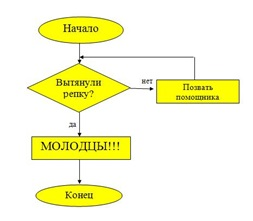
\includegraphics[width=0.63\linewidth]{chapters/chapter28/images/1}
		\caption{}
		\label{ris:image28x1}
	\end{center}
\end{figure}


{\hypertarget{lesson28x3}{\blackBlueText{III. Свободное творчество}}}\\\\	

Каждая команда обсуждает алгоритм будущей программы и рисует соответствующую блок-схему. После одобрения схемы преподавателем команда может приступать к написанию кода.\\\\

{\hypertarget{lesson28x4}{\blackBlueText{IV. Итоги этапа}}}\\\\

Общие результаты шестого этапа, вне зависимости от конкретной задачи, должны выглядеть так:

\begin{itemize}
	\item Сформулированы  все проблемы программной части.
	\item Решены  все  проблемы программной части.
	\item Приведен полный текст программы, соответствующий правилам оформления кода (см. Занятие) и подробно прокомментированный.
\end{itemize}

\noindent\underline{Пример}

ассмотрим, для примера, записи, сделанные по итогам пятой недели в технической книге проектной группы Автобус ФМЛ № 30 ({\slshape курсивом выделены ремарки автора}): 

{\slshape Задача четко сформулирована.}

\noindent\underline{Цель:}~Cоздать автономный автобус, который двигается по чёрной линии, нанесённой на белое поле. Когда автобус попадает в зоны жёлтого цвета, он останавливается, открывает двери, ждёт, пока зайдут пассажиры, закрывает двери и продолжает движение.

{\slshape Алгоритм движения разбит на две части : движение по линии и остановки в желтых зонах. К сожалению, это читателю приходится домысливать, явных указаний на это в технической книге не появилось.}\\\\

\begin{center}
	{\bfseries Движение по линии}
\end{center}

Для движения по линии использован принцип пропорционального регулятора. Чем сильнее робот отклоняется от линии, тем сильнее стремится вернуться обратно с помощью разницы в скоростях моторов.
\clearpage
\begin{figure}[h!]
	\begin{center}
		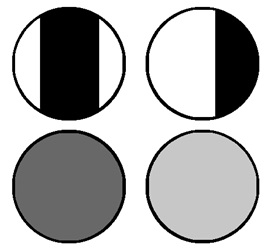
\includegraphics[width=0.84\linewidth]{chapters/chapter28/images/2}
		\caption{Распознавание линии датчиками освещения}
		\label{ris:image28x2}
	\end{center}
\end{figure}

\begin{figure}[h!]
	\begin{center}
		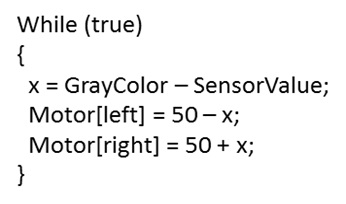
\includegraphics[width=0.84\linewidth]{chapters/chapter28/images/3}
		\caption{Часть программы, отвечающая за движение по линии.}
		\label{ris:image28x3}
	\end{center}
\end{figure}

На рисунке 2 показано, как датчики различают отклонение от линии. На верхних картинках~--- то, что есть на самом деле, на нижних~--- то, что видят датчики.

На рисунке 3 приведена часть программы отвечающая за движение по линии. Полная программа приведена в приложении 1.

Переменной \underline{х} присваивается значение, равное разнице между средним арифметическим значений чёрного и белого цветов и показания датчика. Затем к скорости одного мотора прибавляется значение \underline{х}, а от скорости другого отнимается. Таким образом, чем сильнее отклонение от линии, тем больше разница в скоростях колёс, и тем сильнее робот поворачивает в сторону линии. 

{\slshape Достойный для детского уровня расказ о принципах работы пропорционального регулятора.}

\begin{figure}[h!]
	\begin{center}
		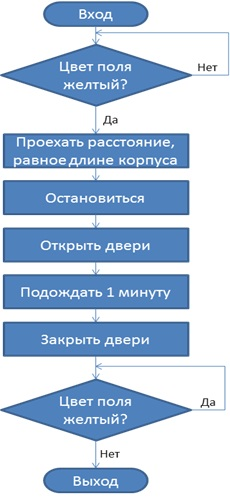
\includegraphics[width=0.4\linewidth]{chapters/chapter28/images/4}
		\caption{Алгоритм остановки в жёлтой зоне}
		\label{ris:image28x4}
	\end{center}
\end{figure}

Последний цикл нужен для того, чтобы робот смог уехать из жёлтой зоны, не делая повторную остановку.
\clearpage
{\slshape С алгоритмом остановки у команды были проблемы. Первоначальная логика программы не имела последнего ветвления. В результате, остановившись на желтом один раз, автобус стоял на нем до бесконечности, открывая и закрывая двери, т.к. цвет фона не менялся. Эта проблема была решена, однако ничего кроме последней строчки о ней в книге не напоминает, что является существенным недостатком. Кроме этого само решение не вполне удачно отображено на блок-схеме выше. Складывается ощущение, что в последнем ветвлении робот может стоять на желтом до бесконечности опять же, тогда как в действительности в процессе проверки этого условия робот непрерывно движется вперед по линии.}\\\\
Полный текст программы:

{\programm
	{\slshape\bC{\#pragma~}\bbC{config}}\rC{(\bbC{\slshape{}Sensor},~\rrC{S1},\indent\indent\bbC{\slshape{}li},\indent\indent\rrC{sensorColorNxtRED})}\\
	\gC{// Строчки, отвечающие}\\
	{\slshape\bC{\#pragma~}\bbC{config}}\rC{(\bbC{\slshape{}Sensor},~\rrC{S2},\indent\indent\bbC{\slshape{}ye},\indent\indent\rrC{sensorColorNxtFULL})}\\
	\gC{// за объявление}\\
	{\slshape\bC{\#pragma~}\bbC{config}}\rC{(\bbC{\slshape{}Motor},~\rrC{motorA},\indent\indent\bbC{\slshape{}bm},\indent\indent\rrC{tmotorNXT},~\bbC{\slshape{}PIDControl},~\bbC{\slshape{}encoder})}\\
	\gC{// датчиков и моторов}\\
	{\slshape\bC{\#pragma~}\bbC{config}}\rC{(\bbC{\slshape{}Motor},~\rrC{motorB},\indent\indent\bbC{\slshape{}lm},\indent\indent\rrC{tmotorNXT},~\bbC{\slshape{}PIDControl},~\bbC{\slshape{}encoder})}\\
	\gC{// и присваивания им}\\
	{\slshape\bC{\#pragma~}\bbC{config}}\rC{(\bbC{\slshape{}Motor},~\rrC{motorC},\indent\indent\bbC{\slshape{}rm},\indent\indent\rrC{tmotorNXT},~\bbC{\slshape{}PIDControl},~\bbC{\slshape{}encoder})}\\
	\gC{// имён и номеров портов}\\\\
	{\slshape\bC{float}}~bl\rC{,}~wh\rC{,}~gr\rC{,}~x\rC{;}\\
	\gC{//Глобальные переменные (использующиеся во всех функциях).}\\\\
	{\slshape\bC{float}}~calibr\rC{()}\\
	\rC{\{}\\
	\indent\gC{//Черный цвет:}\\
	\indent bl~\rC{=~\bbC{SensorValue}[}li\rC{];}\\
	\indent\gC{//Поворот корпуса:}\\
	\indent\bbC{nMotorEncoder}\rC{[}lm\rC{] = \rrC{0};}\\
	\indent\bbC{motor}\rC{[}lm\rC{] = \rrC{30};}\\
	\indent\bbC{motor}\rC{[}rm\rC{] = \rrC{-30};}\\
	\indent{\slshape\bC{while}}\rC{(\bbC{nMotorEncoder}[}lm\rC{] < \rrC{100});}\\
	\indent\bbC{motor}\rC{[}lm\rC{] = \rrC{0};}\\
	\indent\bbC{motor}\rC{[}rm\rC{] = \rrC{0};}\\
	\indent\gC{//Белый цвет:}\\
	\indent wh~\rC{=~\bbC{SensorValue}[}li\rC{];}\\
	\indent\gC{//Среднее арифметическое:}\\
	\indent gr~\rC{=~(}bl~\rC{+}~wh\rC{)~/~\rrC{2};}
	\indent\gC{//Поворот обратно}\\		
	\indent\bbC{nMotorEncoder}\rC{[}lm\rC{] = \rrC{0};}\\
	\indent\bbC{motor}\rC{[}lm\rC{] = \rrC{-30};}\\
	\indent\bbC{motor}\rC{[}rm\rC{] = \rrC{30};}\\
	\indent{\slshape\bC{while}}\rC{(\bbC{nMotorEncoder}[}lm\rC{] > \rrC{-90});}\\
	\indent\bbC{motor}\rC{[}lm\rC{] = \rrC{0};}\\
	\indent\bbC{motor}\rC{[}rm\rC{] = \rrC{0};}\\	
	\indent\bbC{wait1Msec}\rC{(\rrC{1000});}\\
	\rC{\}}\\\\
	{\slshape\bC{task main}}\rC{()}\\
	\rC{\{}\\
	\indent\bbC{wait1Msec}\rC{(\rrC{500});}\\
	\indent calibr\rC{();}\indent\gC{//Вызов функции калибровки}\\
	\indent{\slshape\bC{while}}\rC{(\bC{\slshape true})}\\
	\indent\rC{\{}\\
	\indent\indent{\slshape\bC{while}}\rC{(\bbC{SensorValue}[}ye\rrC{] != \rrC{YELLOWCOLOR})}\\
	\indent\indent\gC{//Пока поле жёлтое, ехать по линии}\\
	\indent\indent\rC{\{}\\
	\indent\indent\indent x~\rC{=~(\bbC{SensorValue}[}li\rC{] -~}gr\rC{)~*~\rrC{2};}\\
	\indent\indent\indent\bbC{motor}\rC{[}lm\rC{] = \rrC{50}~-~}x\rC{;}\\
	\indent\indent\indent\bbC{motor}\rC{[}rm\rC{] = \rrC{50}~+~}x\rC{;}\\
	\indent\indent\rC{\}}\\
	\indent\indent\gC{//Поле стало жёлтым, нужно проехать определённое расстояние:}\\
	\indent\indent\bbC{nMotorEncoder}\rC{[}lm\rC{] = \rrC{0};}\\
	\indent\indent{\slshape\bC{while}}\rC{(\bbC{nMotorEncoder}[}lm\rC{] < \rrC{150})}\\
	\indent\indent\rC{\{}\\
	\indent\indent\indent x~\rC{=~(\bbC{SensorValue}[}li\rC{] -~}gr\rC{)~*~\rrC{2.5};}\\
	\indent\indent\indent\bbC{motor}\rC{[}lm\rC{] = \rrC{50}~-~}x\rC{;}\\
	\indent\indent\indent\bbC{motor}\rC{[}rm\rC{] = \rrC{50}~+~}x\rC{;}\\
	\indent\indent\rC{\}}\\
	\indent\indent\bbC{motor}\rC{[}bm\rC{] = \rrC{50};}\indent\gC{//Открыть дверь}\\
	\indent\indent\bbC{wait1Msec}\rC{(\rrC{5000});}\indent\gC{//Подождать}\\
	\indent\indent\bbC{motor}\rC{[}bm\rC{] = \rrC{-80};}\indent\gC{//Закрыть дверь}\\
	\indent\indent\bbC{wait1Msec}\rC{(\rrC{2000});}\\
	\indent\indent\bbC{motor}\rC{[}bm\rC{] = \rrC{0};}\\
	\indent\indent{\slshape\bC{while}}\rC{(\bbC{SensorValue}[}ye\rrC{] == \rrC{YELLOWCOLOR})}\\
	\indent\indent\rC{\{}\\
	\indent\indent\indent x~\rC{=~(\bbC{SensorValue}[}li\rC{] -~}gr\rC{)~*~\rrC{2};}\\
	\indent\indent\indent\bbC{motor}\rC{[}lm\rC{] = \rrC{50}~-~}x\rC{;}\\
	\indent\indent\indent\bbC{motor}\rC{[}rm\rC{] = \rrC{50}~+~}x\rC{;}\\
	\indent\indent\rC{\}}\\
	\indent\rC{\}}\\
	\rC{\}}\\
}\\	

\noindent Примечание: 

Левый мотор~--- порт B;

Правый мотор~--- порт С;

Дверной мотор~--- порт A;

Датчик RGB`--- порт 2;

Датчик освещённости~--- порт 1.

{\slshape Командой приведен полный текст программы, достаточно подробно прокомментированный. Можно заметить, что в процессе работы над проектом командой были самостоятельно изучены процедуры, что нашло отражение в итоговом коде, написана процедура калибровки. Так же использованы переименования моторов для сокращения объема записей, что так же не рассматривалось в общем курсе. Стоит отметить уместное использование глобальных переменных и констант.
	
Стандартный редактор RobotC не позволяет писать в нем русские символы, таким образом русские комментарии, указывают на то, что писались они уже для отчетности, а не в процессе создания кода. Следует обратить внимание команды на это и еще раз пояснить важность написания комментариев к своей программе.}